 % Template for ICIP-2009 paper; to be used with:
%          spconf.sty  - ICASSP/ICIP LaTeX style file, and
%          IEEEbib.bst - IEEE bibliography style file.
% --------------------------------------------------------------------------
\documentclass{article}
\usepackage{spconf,amsmath,epsfig}
\usepackage{subfigure}
\usepackage{multirow}

% Example definitions.
% --------------------
\def\x{{\mathbf x}}
\def\L{{\cal L}}

% Title.
% ------
\title{COMPENSATION METHODS USING SIGNAL PROCESSING AND ADAPTIVE QUANTIZATION FOR BETTER MEAN SHIFT TRACKING ON COMPRESSED VIDEO}
%
% Single address.
% ---------------
\name{Salman Aslam, Aaron Bobick, Christopher Barnes}
\address{Georgia Institute of Technolgy}
%
% For example:
% ------------
%\address{School\\
%	Department\\
%	Address}
%
% Two addresses (uncomment and modify for two-address case).
% ----------------------------------------------------------
%\twoauthors
%  {A. Author-one, B. Author-two\sthanks{Thanks to XYZ agency for funding.}}
%	{School A-B\\
%	Department A-B\\
%	Address A-B}
%  {C. Author-three, D. Author-four\sthanks{The fourth author performed the work
%	while at ...}}
%	{School C-D\\
%	Department C-D\\
%	Address C-D}
%
\begin{document}
%\ninept
%
\maketitle
%
%--------------------------------------------------------------------------------------------------------------------------------------------------------------
\begin{abstract}
%--------------------------------------------------------------------------------------------------------------------------------------------------------------
In this paper, we discuss methods for coding MPEG-4 video to enable better computer vision on the compressed video. This problem is important since the amount of video content being generated from a variety of sources is increasing very rapidly, almost all this video is in compressed form, and computer vision applications such as video analysis, mining and querying running on these videos are becoming more commonplace.  If the particular computer vision algorithm that is likely to be run on the compressed video is known apriori, then steps can be taken during the encoding process to facilitate the performance of the algorithm.  In this paper, the algorithm we focus on is Mean Shift tracking, a robust and widely used tracker.  We show that by performing signal processing on the input signal before it is encoded, or by adaptively changing the parameters of the encoding process, we can make the resulting signal more robust to degradations in the encoding process.  The result is better tracking on the compressed video, at the same bitrate, but with some loss in PSNR.
\end{abstract}

\begin{keywords}
Computer vision, video compression, surveillance, MPEG-4, Mean Shift tracking
\end{keywords}

%Traditional methods have looked at preferential coding of areas with high motion, or a distinction between foreground and background.  We take this a step further up the analysis ladder and look at motion more  codecs means that more has to be done than to simply create a divide between coding foreground preferentially and giving less importance to background.  
%discuss the general framework entailed in this process.  We then turn to a specific computer vision algorithm on situations where it is known apriori that tracking  will be performed on the compressed video.  We focus on 

%--------------------------------------------------------------------------------------------------------------------------------------------------------------
\section{INTRODUCTION}
%--------------------------------------------------------------------------------------------------------------------------------------------------------------

\subsection{Problem statement}
%-----------------------------
Figure~\ref{fig:ProblemStatement} presents the overall framework we are interested in.  It can be summarized in three points (a) A video signal from a given source needs to be transmitted to another point or stored in some medium. (b) Due to bandwidth or storage limitations, we would like to encode the video. (c) Depending on the application, some measure of information extracted from the original video needs to be preserved in the decoded video. 

\subsection{Motivation}
%----------------------
Examples where the above situation may arise are many.  The increasing trend in video sharing brought on by the popularity of sites such as YouTube~\cite{YouTube} and Facebook~\cite{Facebook} or applications such as MMS, has brought with it novel ways of analysing and mining content.  In these scenarios, computer vision algorithms such as face detection or face finding running on compressed videos from these sources is becoming common.  In more traditional settings, video cameras in surveillance applications normally send back compressed video to a central server for analysis.  Although there is a rising trend in edge processing, i.e. processing at the camera itself, the need to transmit compressed video to a central server for human consumption and data fusion from other sensors still remains important.  Another increasing trend in surveillance applications, usage of live webcams streaming data over the internet, remains relevant to our discussion since these webcams also encode data before transmission.  In satellite imaging applications, compressed video downlinked to ground stations may be analyzed for atmospheric and geological patterns, disaster zone identification, vegetation analysis or structure classification.  In medical imaging, there is a rising trend in remote diagnosis and surgery, with compressed video being sent to doctors in remote locations. 

			%figure: problem statement
			\begin{figure}				
					\includegraphics[width=.45\textwidth]{figs/TRK_IPCV2009_BlockDiagram_1}
					\caption{Information in the decoded video must be close in some sense to information in the original video.}
					\label{fig:ProblemStatement}
			\end{figure}

\subsection{Possible Approaches}
%-------------------------------
In the applications mentioned above, and in hundreds of other applications where it is important to preserve some measure of information in the video signal other than visual quality, the goal of coding video can be addressed in the following ways,

\begin{itemize}

\item \textbf{Specific codec for every application.} Design a video codec tailored for each application that efficiently concentrates bits where they matter most.  The disadvantages in terms of cost, maintainability, upgradeability and cross operability are obvious.

\item \textbf{Standard codec with metadata.}  Provide a general framework for transmitting both video and information extracted from the video in a coherent and integrated manner as part of the codec specification.  This approach was adopted by MPEG in 1993 and resulted in MPEG-4.  However, in practice, the scene construction and description features of this standard did not gain much acceptance.

\item \textbf{Standard codec.}  Use standard universally accepted rectangular based MPEGx and H.26x codecs and change their parameters during the encoding process to preserve the desired information.  We call this approach $VarPar$ (variable parameter) compensation.

\item \textbf{Signal processing on the input.}  In places where access to the encoding process is not available or not desired, apply signal processing on the input signal to make it more robust to degradations during the encoding process.  We call this approach $SigProc$ (signal processing) compensation.

\end{itemize}

			%figure: general solution

			\begin{figure}
						\centering
						\includegraphics[width=.45\textwidth]{figs/TRK_IPCV2009_BlockDiagram_2_VarPar}
						\caption{Encoder $VarPar$ (variable parameter) compensation.}
						\label{fig:SolutionThroughVarPar}
			\end{figure}

			\begin{figure}
						\centering
						\includegraphics[width=.45\textwidth]{figs/TRK_IPCV2009_BlockDiagram_2_sigProc}
						\caption{$SigProc$ (signal processing) compensation.}
						\label{fig:SolutionThroughSigProc}
			\end{figure}

			%experimental setup
			\begin{figure}
					\includegraphics[width=.45\textwidth]{figs/TRK_IPCV2009_ExperimentalSetup_sigProc_VarPar}
					\caption{Experimental setup.}
					\label{fig:ExperimentalSetup}
			\end{figure}

We are not interested in the first two methods discussed above due to their limitations.  We now discuss $VarPar$ and $SigProc$ compensation in the following paragraphs.

\subsubsection{VarPar Compensation}
This approach is depicted in Figure~\ref{fig:SolutionThroughVarPar}.  In this approach, the encoding parameters are adjusted adaptively based on the input signal to maximize some measure of information in the input signal.  $VarPar$ compensation has been used in the literature for computer vision algorithms that rely on motion.  In such cases, researchers have preferentially encoded areas with high motion, or in more sophisticated cases, preferentially encoded the foreground~\cite{2005_CNF_SceneAnalysisForJPEG2000_Meessen}.  Very little literature is available for computer vision algorithms that do not rely on motion. 

\subsubsection{SigProc Compensation}
This approach is depicted in Figure~\ref{fig:SolutionThroughSigProc}.  Very little literature is available on this approach.  The idea here is to transform the input signal so that it better preserves some measure of information as it undergoes distortions in the encoding process.  $SigProc$ can be applied in two ways:

\begin{itemize}
\item {No inverse signal processing required.}  Signal processing can be applied on the input signal so as to maximize a similarity measure between input and output.  In such cases, the output signal will remain intelligible to a human observer.  This is important where no further processing after the decoding process is desired.

\item {Inverse signal processing required.}  In cases where human consumption of the decoded signal is not required, or where extra processing after the decoding step is possible, one may apply signal processing to severely distort the input signal in a way that it better preserves some measure of information during the encoding process.  MPEGx and H.26x, the two prevalent standard video coding standards compress video so that low frequency scene reconstruction elements most useful for the human visual system remain preserved.  One can then try to process the input signal so that desired information content is encoded at lower frequencies.

%PETS2001
\begin{figure}%[htp]
			\centering

			\subfigure[Ground truth]
				{
					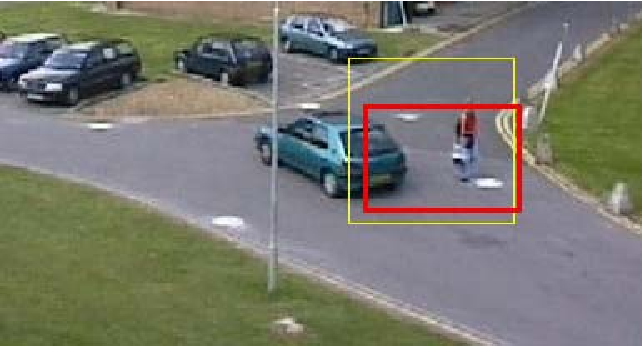
\includegraphics[width=.22\textwidth]{figs/TRK_IPCV2009_PETS2001_FN_00592_outputGroundTruth}
					\label{fig:PETS2001_Frame592_Ground}
				}
			\subfigure[Base]
				{
					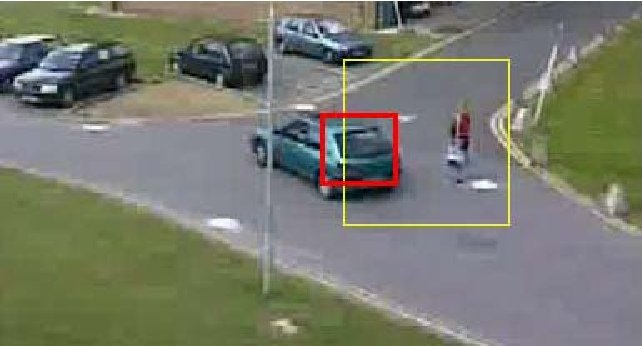
\includegraphics[width=.22\textwidth]{figs/TRK_IPCV2009_PETS2001_FN_00592_outputBaseline}
					\label{fig:PETS2001_Frame592_Base}
				}
			\subfigure[SigProc]
				{
					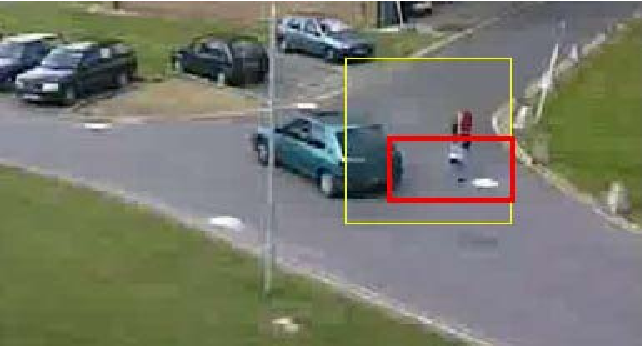
\includegraphics[width=.22\textwidth]{figs/TRK_IPCV2009_PETS2001_FN_00592_outputSigProc}
					\label{fig:PETS2001_Frame592_SigProc}
				}
			\subfigure[VarPar]
				{
					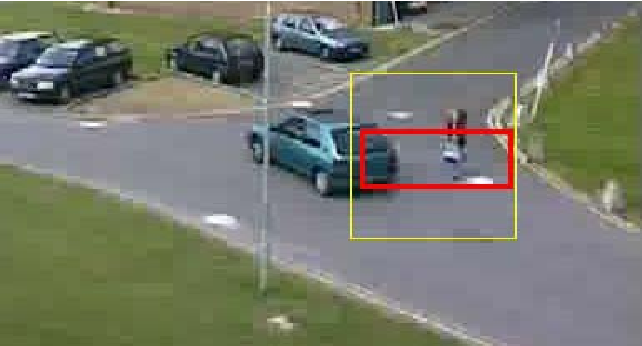
\includegraphics[width=.22\textwidth]{figs/TRK_IPCV2009_PETS2001_FN_00592_outputVarPar}
					\label{fig:PETS2001_Frame592_VarPar}
				}	
			\caption{PETS2001} 	
			\label{fig:PicsPETS2001}	
\end{figure}

More formally, $SigProc$ can be cast as a calculus of variations problem where we seek to minimize the functional J(g)

\begin{equation}
\label{eq:CalcOfVarFormulation}
J(g)=\int\int_D \left\|f(I) - f(\hat{g}(I)) \right\|  +  \left\|p(I) - p(\hat{g}(I)) \right\| dxdy
\end{equation}

$\hat{g}(I)$ can be written as $C^{-1}(C(g(I(x,y)))$ where $C(x,y)$ is 

\begin{equation}
\label{eq:DCT}
C(x,y) = \sum_{x_0}\sum_{y_0}T(Q(D(I)))\delta(x-kx_0, y-ky_0)
\end{equation}

Here $I(x,y)$ is the original image.  $D(x,y)$ is the DCT transform of a $kxk$ block of image data or motion compensated residuals.  The value of $k$ is normally 8.  $Q(x,y)$ is a quantization function and can depend on quantization matrices and the quantization parameter $Qp$. $T(x,y)$  is a thresholding function.  We omit the lossless parts of the compression system, such as Huffman Coding, Arithmetic Coding etc, since they do not result in distortions in our setup.  There is an additional element of numerical precision errors, particularly in the DCT setup that we choose to ignore for simplicity.  $f(x,y)$ is the computer vision algorithm that we're interested in.

Equation~\ref{eq:CalcOfVarFormulation} then says that over the space of all transformations that can be applied to the input image $I(x,y)$, we would like to find the signal processing function $g(x,y)$ that minimizes the distance between the output of a computer vision algorithm $f(x,y)$ running on the original image and running on the compressed image, and that also maximizes some similarity measure $p(x,y)$ of the image.  It is clear that Equation~\ref{eq:CalcOfVarFormulation} is not differentiable due to the discontinuities on the $kxk$ DCT block boundaries.  However, even if numerical schemes are resorted to, the Euler Lagrange approach to solving the variational problem is a necessary but not sufficient condition for global optimality.  In such cases, one can resort to finding a signal processing function $g(x,y)$ either experimentally through Monte Carlo simulations, or using prior knowledge of the nature of the computer vision algorithm we are interested in.

%PETS2007
\begin{figure}%[htp]
			\centering

			\subfigure[Ground truth]
				{
					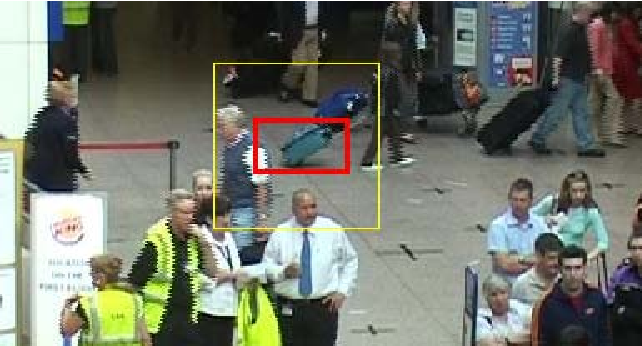
\includegraphics[width=.22\textwidth]{figs/TRK_IPCV2009_PETS2007_FN_00340_outputGroundTruth}
					\label{fig:PETS2007_Frame340_Ground}
				}
			\subfigure[Base]
				{
					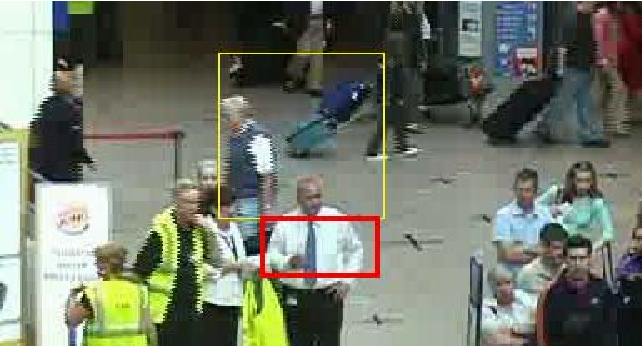
\includegraphics[width=.22\textwidth]{figs/TRK_IPCV2009_PETS2007_FN_00340_outputBaseline}
					\label{fig:PETS2007_Frame340_Base}
				}
			\subfigure[SigProc]
				{
					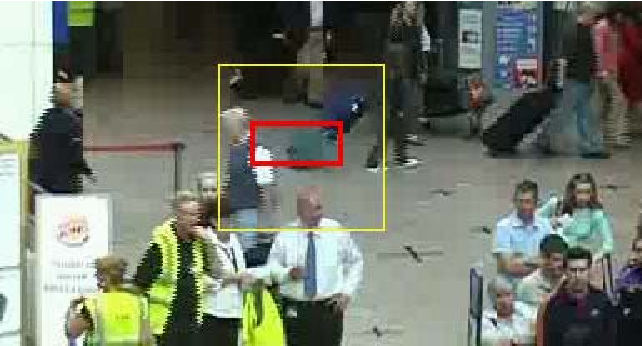
\includegraphics[width=.22\textwidth]{figs/TRK_IPCV2009_PETS2007_FN_00340_outputSigProc}
					\label{fig:PETS2007_Frame340_SigProc}
				}
			\subfigure[VarPar]
				{
					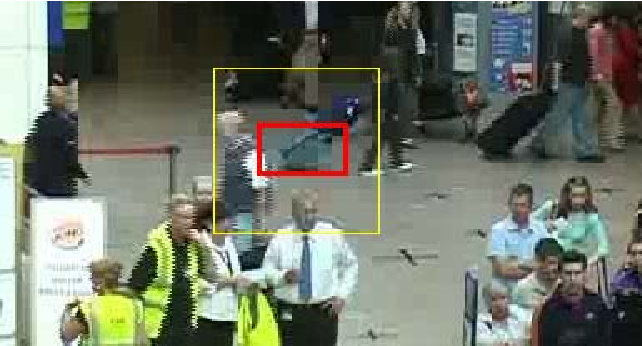
\includegraphics[width=.22\textwidth]{figs/TRK_IPCV2009_PETS2007_FN_00340_outputVarPar}
					\label{fig:PETS2007_Frame340_VarPar}
				}	
			\caption{PETS2007}
			\label{fig:PicsPETS2007} 		
\end{figure}

%Without loss of generality, we use I frames and therefore the DCT transform is for $kxk$ blocks of image data.


%--------------------------------------------------------------------------------------------------------------------------------------------------------------
\section{EXPERIMENTS}
%--------------------------------------------------------------------------------------------------------------------------------------------------------------
After having discussed the general approaches to our problem, we now discuss the specific approach that we use in this paper.  The computer vision algorithm that we use is Mean Shift tracking.  Before proceeeding with other specifics of our approach, we give an overview of this algorithm.

\begin{align}
	\label{eq:MeanShiftEquations}
	M_{00}&=\sum_x\sum_yI(x,y)\notag\\
	M_{10}&=\sum_x\sum_yxI(x,y)\notag\\
	M_{01}&=\sum_x\sum_yyI(x,y)\\
	x_c&=\frac{M_{10}}{M_{00}}\notag \\
	y_c&=\frac{M_{01}}{M_{00}} \notag
\end{align}

\subsection{Theory: Mean Shift Tracking}
%---------------------------------------
The goal of the Mean Shift algorithm is to find the peak of a distribution over time  \cite{2003_JNL_TRKkernel_Comaniciu}.  An initial reference histogram is created in some desired space, of the object to be tracked.   After creating the initial histogram, subsequent images are backprojected on this histogram to create a likelihood function.  A window placed over the initial location of the target object is then placed on this backprojected window and moved to a new place as computed by the mean shift vectors, $x_c$ and $y_c$ (Equation~\ref{eq:MeanShiftEquations}).  If a rectangular kernel for the window is used \cite{1998_JNL_FaceObjectTracking_Bradski}, \cite{2008_BOOK_OpenCV_Bradski}, then the mean shift computations reduce to finding the zeroth and first order image moments as shown in Equation~\ref{eq:MeanShiftEquations}.  This step is repeated until the mean shift vectors converge.  

%accuracy
%--------
			\begin{figure}%[htp]
				\centering
				
				\subfigure[PETS2001]
					{
						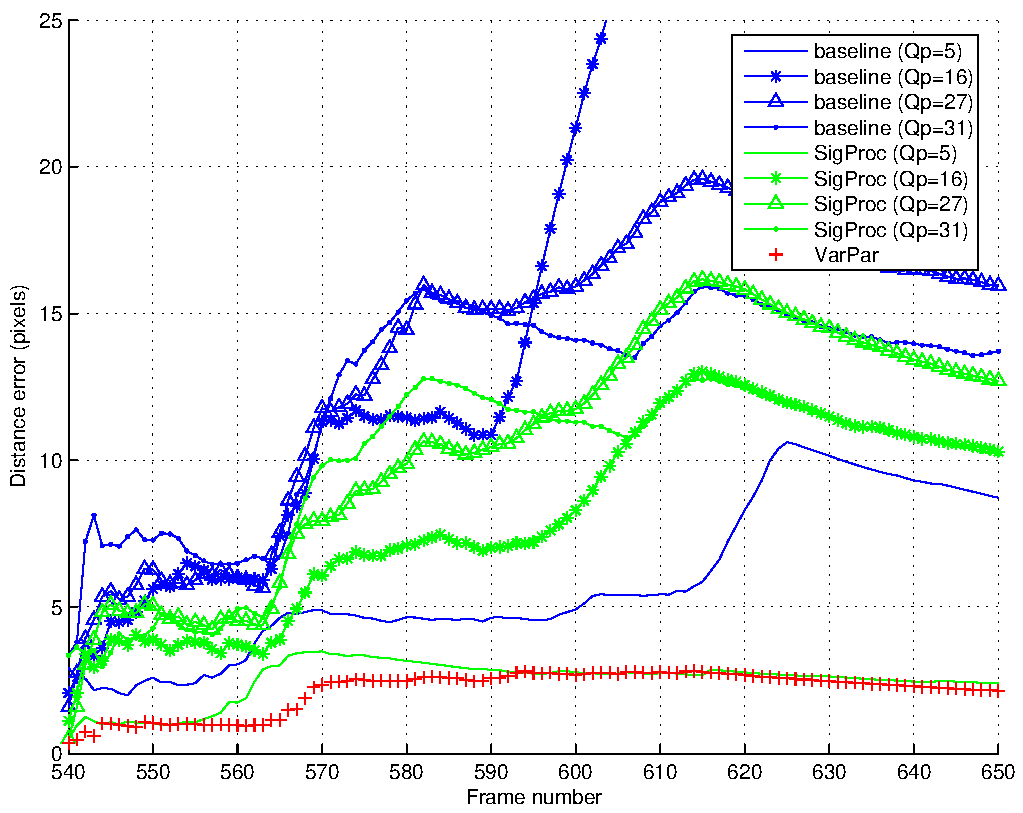
\includegraphics[width=.45\textwidth]{figs/TRK_IPCV2009_PETS2001_TrackingError}
						\label{fig:Accuracy_PETS2001}
					}
				\subfigure[PETS2007]
					{
						\includegraphics[width=.45\textwidth]{figs/TRK_IPCV2009_PETS2007_TrackingError}
						\label{fig:Accuracy_PETS2007}
					}
					
				\caption{Tracking accuracy.} 		
				
			\end{figure}



\subsection{Components Of Experimental Setup}
%--------------------------------------------
Our experimental setup is given in Figure~\ref{fig:ExperimentalSetup}.  The different components in this setup are explained below.


%quality
%--------
			\begin{figure}[t]
				\centering
				
				\subfigure[PETS2001]
					{
						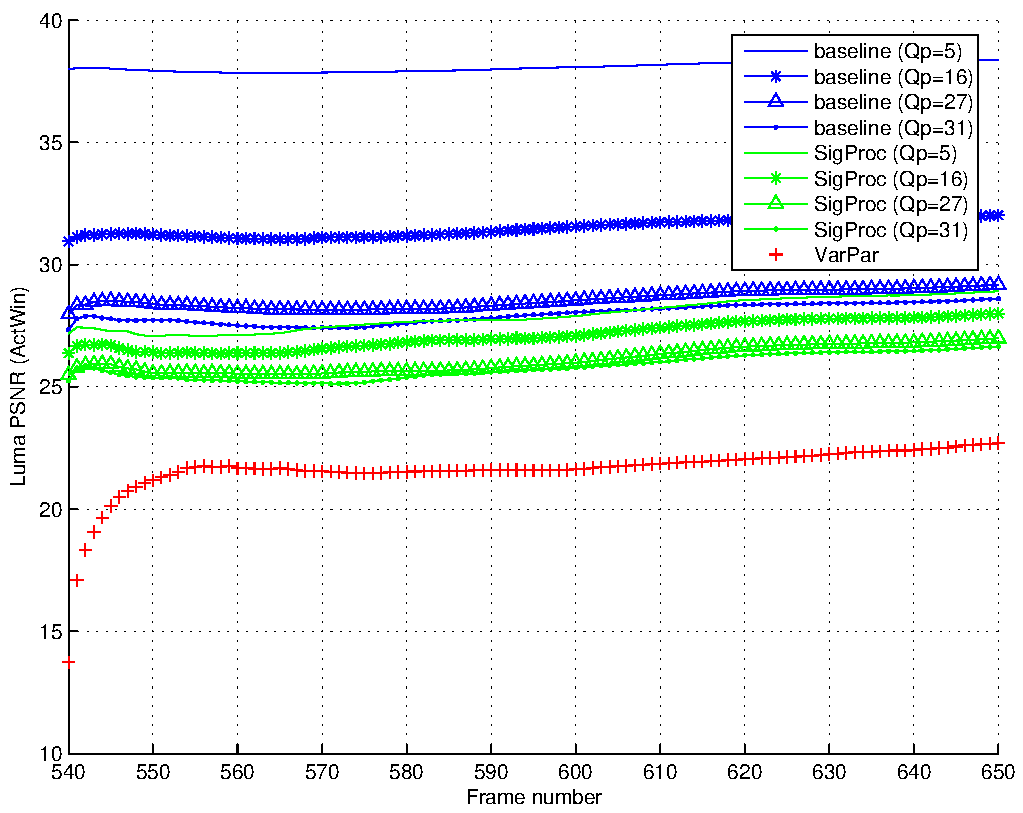
\includegraphics[width=.45\textwidth]{figs/TRK_IPCV2009_PETS2001_PSNRinROI}
						\label{fig:Quality_PETS2001}
					}
				\subfigure[PETS2007]
					{
						\includegraphics[width=.45\textwidth]{figs/TRK_IPCV2009_PETS2007_PSNRinROI}
						\label{fig:Quality_PETS2007}
					}
					
				\caption{PSNR comparison in $ActWin$.} 		
				
			\end{figure}	

\begin{itemize}
\item \textbf{Input data.}  For the input data, we used image sequences from two standard databases, PETS2001 and PETS2007 (Performance Evaluation of Tracking and Surveillance).  In PETS2001, we track a person in a sparse background as she gets occluded by a car with a similar color distribution.  In PETS2007, we track a bag in a dense environment.  These two scenarios were chosen since they are quite different from each other and would provide a better test of our approach.  Additionally, in both cases, the tracked object is occluded by another object with a similar color distribution.  This of course, presents one of the most significant challenges in tracking applications.   
\item \textbf{Computer vision algorithm.}  As mentioned earlier, the specific computer vision algorithm that we chose to experiment with is the Mean Shift tracker.  The implementation used is from the standard open source Intel OpenCV library.  The feature distribution used is the hue component of the HSV space.  Convergence takes 3 to 4 steps on the original and compensated images and up to 8 to 9 steps for the uncompensated images.  We manually initialize the object to be tracked.  In the case of static cameras, it could come from a background modeling process such as the Multi Gaussian algorithm~\cite{2000_JNL_MG_Stauffer},~\cite{2005_JNL_SURVEYchangeDetection_Radke}.  However, we make no assumptions about this step, and our approach is equally valid for moving cameras. 

%quantity
%--------
			\begin{figure}[t]
				\centering
				
				\subfigure[PETS2001]
					{
						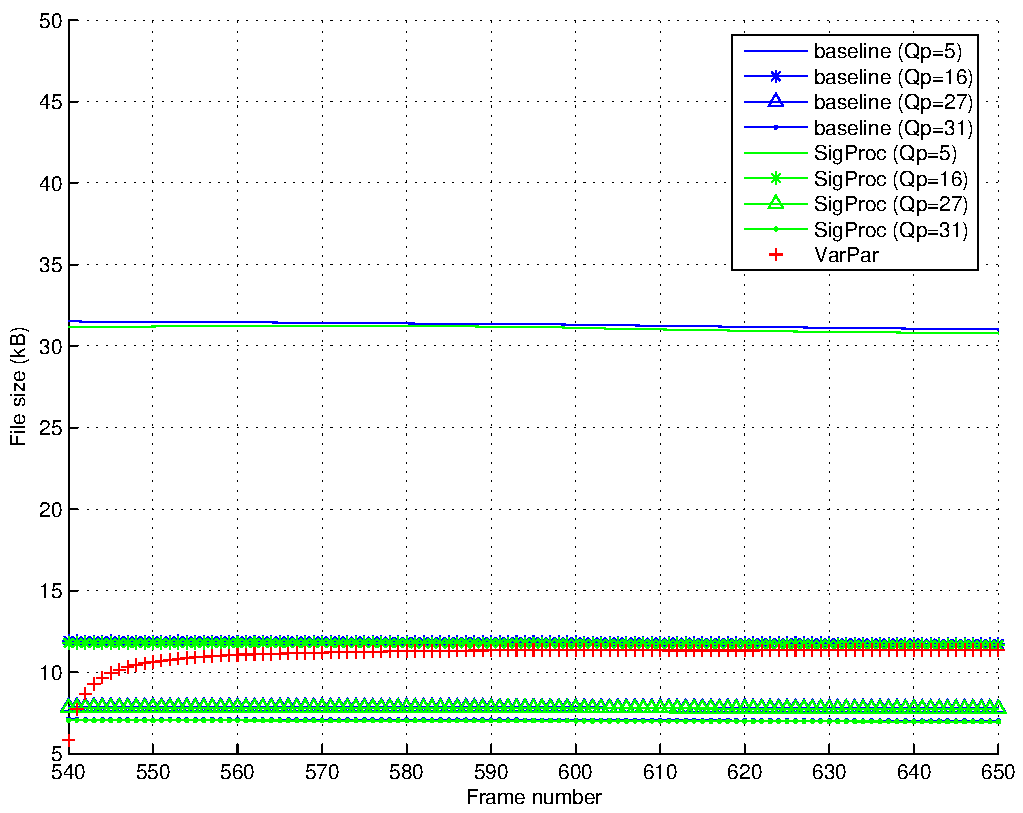
\includegraphics[width=.45\textwidth]{figs/TRK_IPCV2009_PETS2001_fileSizekB}
						\label{fig:Quantity_PETS2001}
					}
					
				\subfigure[PETS2007]
					{
						\includegraphics[width=.45\textwidth]{figs/TRK_IPCV2009_PETS2007_fileSizekB}
						\label{fig:Quantity_PETS2007}
					}
					
				\caption{File size comparison.} 		
				
			\end{figure}	

%accuracy (3D)
%-------------
			\begin{figure}[t]
				\centering
				
				\subfigure[PETS2001]
				{	
					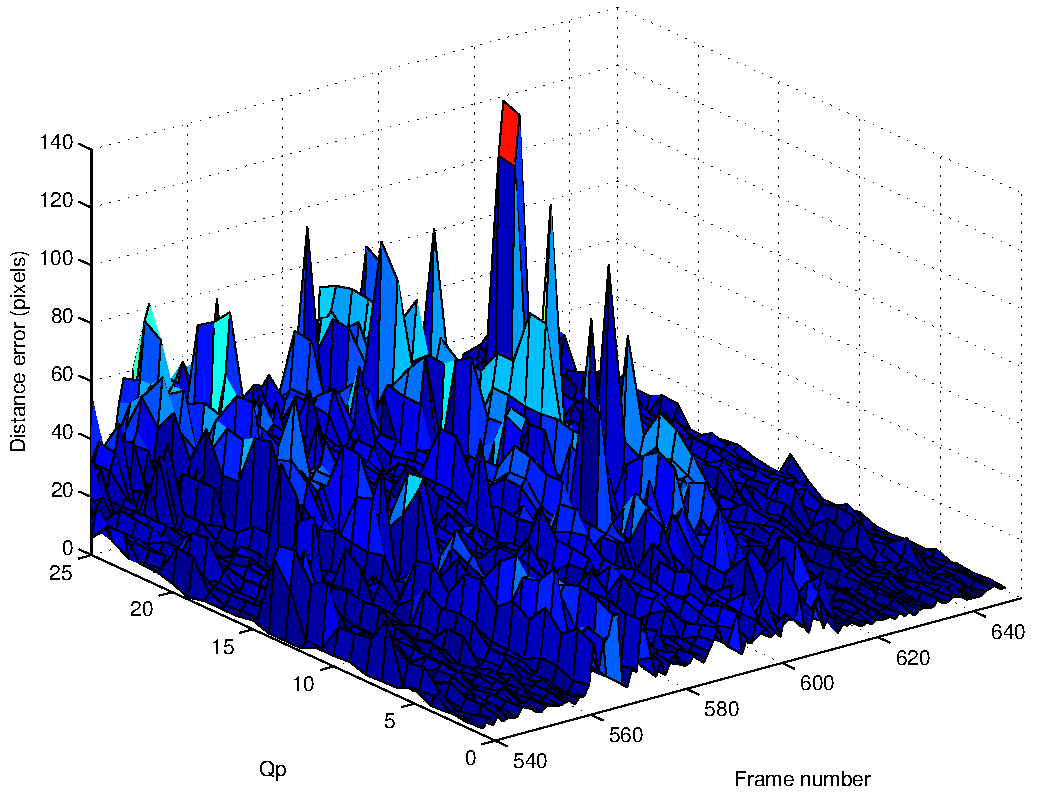
\includegraphics[width=.45\textwidth]{figs/TRK_IPCV2009_PETS2001_TrackingError3D}
					\label{fig:Accuracy_PETS2001_3D}
				}
				
				\subfigure[PETS2007]
				{	
					\includegraphics[width=.45\textwidth]{figs/TRK_IPCV2009_PETS2007_TrackingError3D}
					\label{fig:Accuracy_PETS2007_3D}
				}
				\caption{$VarPar$, tracking accuracy at different values of $Qp$.}
				\label{fig:3D}
			\end{figure}

\item \textbf{Codec.}  The codec used is a standard MPEG-4 Part 2 Visual codec obtained from ISO.  The reason for not using an H.264 codec is that some of our initial experiments tried to use object based functionality of this codec, which is not provided in H.264.  
\item \textbf{Compensation methods.}  The compensation methods, as discussed above were $SigProc$ and $VarPar$, both applied independently.  $SigProc$ was applied in a way to maximize similarity with the input image so that no further processing would be required after the decoder.
\item \textbf{Outputs.}
\begin{itemize}
\item \underline{Ground truth:}  Ground truth tracking output was obtained by running Mean Shift tracking on the input sequences.
\item \underline{Baseline:}  Baseline tracking output was obtained by running Mean Shift tracking on MPEG-4 coded input sequences.  The quality of the video was changed using the quantization parameter $Qp$.  Quantization matrices were not adjusted.  $Qp$ was adjusted to take on one of the following 4 values: 5, 16, 27 and 31.  
\item \underline{$SigProc$ output:}  $SigProc$ tracking output was obtained by running Mean Shift tracking on MPEG-4 coded, signal processed, input sequences.  The signal processing algorithm that we picked is Mean Shift segmentation, which uses the same technique as the Mean Shift tracker to center its window on local histogram peaks.  At this stage, we made three decisions.  First, the class of the signal processing algorithm to be used, i.e. segmentation.  Second, the particular algorithm within the class, i.e. Mean Shift segmentation.  Third, for the parameters of the algorithm, we iterated over the process of segmentation, compression, decompression, tracking, comparing results with the ground truth, and then choosing segmentation parameters that produce the best results.  All this was done automatically.  The reason for choosing Mean Shift segmentation was that since the Mean Shift tracker needs the backprojected window to compute its motion vectors, Mean Shift segmentation should provide a better backprojection.  Even though that backprojection would undergo distortions through the MPEG-4 codec, it would still better preserve local hue information.  We did not segment the whole image, but only a window placed around the object of interest.  This window is different from the Mean Shift tracker window and is called the Active Window, or $ActWin$ hereafter, for clarity.  $ActWin$ was initialized in the same step as the Mean Shift tracker, and from there on, its position was updated automatically.  
\item \underline{$VarPar$ output:}  $VarPar$ tracking output was obtained by running Mean Shift tracking on MPEG-4 coded input sequences.  $Qp$ was iterated over inside $ActWin$ and the best $Qp$ chosen to encode the area inside $ActWin$.  The $Qp$ for the rest of the image outside $ActWin$ was kept same as for the baseline sequence.
\end{itemize}
\item \textbf{Metrics.}  We compare tracking performance for $SigProc$ and $VarPar$ with baseline tracking output using 3 metrics:
\begin{itemize}
\item \underline{Performance.}  This is a comparison with baseline Euclidean distance from ground truth (of bounding box center, measured in pixels).
\item \underline{Quality.}  This is a comparison with baseline PSNR inside $ActWin$.
\item \underline{Bandwidth/bitrate.}  This is a comparison with baseline Intra coded file size.
\end{itemize}
\end{itemize}
%--------------------------------------------------------------------------------------------------------------------------------------------------------------
\section{RESULTS}
%--------------------------------------------------------------------------------------------------------------------------------------------------------------
\end{itemize}
\begin{table}
\centering
\begin{tabular}{|l|c|c|c|c|}
\hline
\multicolumn{5}{|c|}{Accuracy} \\
\hline
Dataset & Qp & Baseline & $SigProc$  & $VarPar$\\ 
\hline
\multirow{4}{*}{PETS2001} 
	&5  & 8.7 	&   2.4 &   2.1 \\
	&16 & 75.4 &  10.3 &   2.1\\
	&27 &16.0 	&  12.7 &   2.1\\
	&31 &13.7 &  10.2 &   2.1\\
\hline
\multirow{3}{*}{PETS2007} 
	&5 &5.8 &   3.5 &   1.0\\
	&16 &85.1 &   4.2 &   1.0\\
	&27 &71.8 &   3.5 &   1.0\\
	&31 &15.2 &  35.8 &   1.0\\
\hline
\multirow{1}{*}{Average}
& - & 36.5 & 10.3 & 1.6 \\  
\hline
\end{tabular}
\caption{Distance from ground truth.}
\label{tab:Accuracy}
\end{table}

\begin{table}
\centering
\begin{tabular}{|l|c|c|c|c|}
\hline
\multicolumn{5}{|c|}{Quality} \\
\hline
Dataset & Qp & Baseline & $SigProc$  & $VarPar$\\ 
\hline
\multirow{4}{*}{PETS2001} 
	&5 &38.4 &  28.9 &  22.7\\
	&16 &32.0 &  28.0 &  22.7\\
	&27 &29.2 &  27.0 &  22.7\\
	&31 &28.6 &  26.6 &  22.7\\
\hline
\multirow{3}{*}{PETS2007} 
	&5 &37.4 &  26.6 &  26.8\\
	&16 &29.9 &  25.7 &  26.8\\	
	&27 &27.3 &  24.9 &  26.8\\
	&31 &26.1 &  23.9 &  26.8\\
\hline
\multirow{1}{*}{Average}
& - & 31.1 & 26.45 & 24.72 \\ 
\hline
\end{tabular}
\caption{PSNR(dB).}
\label{tab:Quality}
\end{table}

\begin{table}
\centering
\begin{tabular}{|l|c|c|c|c|}
\hline
\multicolumn{5}{|c|}{Bitrate} \\
\hline
Dataset & Qp & Baseline & $SigProc$  & $VarPar$\\ 
\hline
\multirow{4}{*}{PETS2001} 
	&5 &31.0 &  30.8 &  -\\
	&16 &11.7 &  11.6 &  11.3\\
	&27 &7.8 &   7.7 &  -\\
	&31 &7.0 &   7.0 &  -\\
 \hline
 \multirow{3}{*}{PETS2007} 
	&5 &48.4 &  48.0 &  -\\
	&16 &18.3 &  18.2 &  17.9\\
	&27 &11.3 &  11.3 &  -\\
	&31 &9.9 &   9.8 &  -\\
\hline
\multirow{1}{*}{Average}
& - & 18.2 & 18.0 & - \\ 
\hline
\end{tabular}
\caption{File sizes.}
\label{tab:FileSize}
\end{table}

Tracking results are given in Tables~\ref{tab:Accuracy},~\ref{tab:Quality} and~\ref{tab:FileSize}.  Table~\ref{tab:Accuracy} shows the Euclidean distance in pixels, of bounding box centers, produced by the baseline, $SigProc$ and $VarPar$ outputs.  We can see that compared to the baseline, $SigProc$ produces 3.5 times and $VarPar$ produces 22.8 times more accurate results.  This increased accuracy comes at a price.  Table~\ref{tab:Quality} shows that price.  We see that $SigProc$ loses 4.65 dB inside $ActWin$ compared with the baseline, while $VarPar$ loses 6.38 dB.  As far as file size is concerned, which we use as an estimate of the bitrate, $SigProc$ has 0.99 of the baseline's bitrate, while $VarPar$ has 0.97 of the baseline's bitrate.  Comparison of $VarPar$ is at $Qp=16$ as shown in Table~\ref{tab:FileSize}.  So the tradeoff is not in terms of bitrate, where $SigProc$ and $VarPar$ actually do better but in terms of PSNR inside $ActWin$. 
 
In Figures~\ref{fig:Accuracy_PETS2001} and ~\ref{fig:Accuracy_PETS2007}, Figures~\ref{fig:Quality_PETS2001} and ~\ref{fig:Quality_PETS2007} and Figures~\ref{fig:Quantity_PETS2001} and ~\ref{fig:Quantity_PETS2007}, we show accuracy, PSNR and filesize for PETS2001 and PETS2007 respectively plotted against time, i.e. frames.  As far as accuracy results are concerned, it is clear from these figures that $VarPar$ consistently does better than the baseline.  $SigProc$, does better than the baseline in all but one situation.  This situation is shown in Figure~\ref{fig:Accuracy_PETS2007} for $Qp=31$.  The reason is that the bag being tracked is occluded by a person with a similar color distribution.  At some values of $Qp$, part of the object being tracked and part of the occluding object which end up in the same macroblock, may be coded uniformly throwing the tracker of course.  This presents a fundamental challenge in block based codecs since the block boundaries are not aligned with the computer vision algorithm boundaries.

Figures~\ref{fig:PicsPETS2001} and~\ref{fig:PicsPETS2007} show situations in the tracking sequence where the baseline tracker is thrown off track while $SigProc$ and $VarPar$ hold track.  The baseline tracker looses track in Figure~\ref{fig:PicsPETS2001} as the woman emerges from behind a car whose color distribution has some elements close to her own distribution.  A similar situation is shown in Figure~\ref{fig:PicsPETS2007} as the blue bag emerges from behind a man wearing a blue sweater.  The tracker then locks on to a blue tie.  The target bounding box is shown in red, while the $ActWin$ boundary is shown in yellow.  

Figure~\ref{fig:3D} shows the tracking accuracy of $VarPar$ as it iterates over values of $Qp$ in $ActWin$.  The best value of $Qp$ is picked.  It is clear that the tracking doesn't necessarily get worse at higher values of $Qp$, which is interesting.  
\\

%--------------------------------------------------------------------------------------------------------------------------------------------------------------
\section{CONCLUSIONS}
%--------------------------------------------------------------------------------------------------------------------------------------------------------------
Our goal in this paper was to understand how to make a video signal robust to degradations in the encoding process with respect to some information measure extracted by a computer vision algorithm.  In this paper, we used the Mean Shift tracker as the computer vision algorithm.  We used two methods $SigProc$, signal processing on the input video signal, and $VarPar$, variable parameters of the encoder, to achieve this purpose.  In both cases we saw that tracking accuracy improved, albeit at a loss in PSNR.  It is now up to the application at hand to see if the tradeoff is justifiable.  We on our part, will experiment with a broader class of computer vision algorithms, a broader class of compensation schemes, and a larger variety of datasets.

%--------------------------------------------------------------------------------------------------------------------------------------------------------------
%BIBLIOGRAPHY
%--------------------------------------------------------------------------------------------------------------------------------------------------------------
\bibliographystyle{IEEE}
\bibliography{c:/salman/work/writing/MyCitations}

\end{document}
